\documentclass[openany, longbibliography,slovene,a4paper,12pt]{article}
\usepackage[a4paper,inner=3.5cm,outer=2.5cm,top=2.5cm,bottom=2.5cm]{geometry}

\usepackage{braket}
\usepackage{float}
\usepackage{afterpage}
\usepackage{graphicx}
\usepackage{amssymb}

\usepackage[tbtags]{amsmath}
\usepackage[T1]{fontenc}
\graphicspath{{./slike/}{../slike_vezikel_z_robom/}{/home/jure/sola/magisterij/uporabljene_slike/}
{../eps_pdf/}}
\DeclareGraphicsExtensions{.eps,.jpeg,.png,.gif,.pdf}
\usepackage[outdir=./slike/]{epstopdf}
\epstopdfsetup{
	suffix=,
}
\usepackage[multidot]{grffile}

%\usepackage[slovene]{babel}      % slovenski delilni vzorci (!)
%\usepackage[english]{babel}
\usepackage[utf8]{inputenc}
\usepackage{makeidx}
\usepackage{enumerate}
\usepackage{caption}
\usepackage{subcaption}
\usepackage[tbtags]{mathtools}

\usepackage[section]{placeins}

\usepackage[hyphens,spaces,obeyspaces]{url}
\usepackage{breakurl}


\usepackage{ragged2e}
\edef\UrlBreaks{\do\-\UrlBreaks}

\usepackage{makeidx}
\pagestyle{headings}
\makeindex
\usepackage{fancyhdr}
\usepackage[titletoc,title]{appendix}


\usepackage[sort, numbers]{natbib}
\usepackage[pdfa]{hyperref}
\usepackage[x-1a]{pdfx}
\usepackage{pdfpages}
\usepackage{breqn}


\DeclareMathOperator{\arcsinh}{arcsinh}

\def\epsfg#1#2{\epsfig{file=#1.eps,width=#2}}
\def\legendamp#1#2{\vbox{\hsize=#1\caption{\small #2}}}

\setcounter{topnumber}{4}
\setcounter{bottomnumber}{4}
\setcounter{totalnumber}{5}
\renewcommand{\topfraction}{0.99}
\renewcommand{\bottomfraction}{0.99}
\renewcommand{\textfraction}{0.0}
\setlength{\tabcolsep}{10pt}
\renewcommand{\arraystretch}{1.5}

\def\bi#1{\hbox{\boldmath{$#1$}}}
\let\oldvec\vec
\def\vec#1{\mbox{\boldmath$#1$}}
\def\pol{{\textstyle{1\over2}}}
\def\svec#1{\mbox{{\scriptsize \boldmath$#1$}}}

\newcommand{\dif}{\mathrm{d}}
\usepackage{xparse}
\DeclareDocumentCommand{\myint}{o m o o}  
{%
	\int \IfValueT{#1}{#1} \dif #2 \IfValueT{#3}{\dif#3} \IfValueT{#4}{\dif#4}
}
\newcommand{\Alpha}{A}
\newcommand{\Beta}{B}
\newcommand{\Epsilon}{E}
\newcommand{\Kappa}{K}


\begin{document}
\section{Introduction}
One of the most important basic problems in physics is the dynamics of many-body system. Specificaly, in quantum physics and chemistry, the dynamics of electrons and their spatial distribution determine the stability of matter. But it is not just the stability that matters. Electronic structure of materials determines many macroscopic properties like thermal and electrical conductivity, their response to electronic and magnetic field, etc.

Calculation of electronic structure has always been a challenge. It quickly became apparent that direct use of schroedinger equation is not a realistic prospect for calculation of electronic structure, except for some small molecules, as it's time complexity grows exponentially as a function of electron number. With the development of computers different numerical schemes for computation of electronic structure and optimization of molecular structure have emerged. One of them is also density functional theory (DFT from now on), which has been known for roughly 50 years. Through the years DFT has developed and today it represents one of the main tools for calculation of electronic structure especially for complex molecules and crystals.

\section{Matter description}
Physical description of matter surrounding us is given by hamiltonian:
\begin{equation}
H=T_n + T_e + W_{n-n} + W_{e-e} + W_{n-e} + V_{ext},
\end{equation}
where $T_n$ and $T_e$ are kinetic energies of nuclei and electrons respectively, $W_{n-n}$, $W_{e-e}$ and $W_{e-n}$ represent  nuclei-nuclei, electron-electron and electron-nuclei interaction terms. $V_ext$ represents external potential. Ground state of such system is given by the solution of time independant Schroedinger equation:
\begin{equation}
\hat H \psi = \epsilon_0 \psi_0,
\end{equation} 
where index $0$ denotes the solution with the lowest energy. In general $\psi_0$ depends on $3N$ coordinates, where $N$ is total number of particles. This means that complex systems with more than e.g. 10 atoms are very computationally demanding. It is common to reduce the dimensionality of the problem by employing Born-Oppenheimer approximation in which nuclei have fixed positions.

\section{Density functional theory}
DFT is a method, which allows us to replace operator, which operate on
wavefunctions, with operators which depend only on density of particles of
particular spin. The core of dft lies in Kohn-Sham theorems. These two theorems
ensure that stationary many-particle systems are fully characterized by their
ground state density. For non-degenerate case the latter is uniquely determined
by many-particle wave function, which in turn is uniquely determined by the
external potential. For a simple non-degenerate case we will prove this theorem. Let us consider hamiltonian of the form:
\begin{equation} \label{ks_hamiltonian}
\hat H = \hat T + \hat W + \hat V_{ext},
\end{equation}
where $T$ is kinetic energy, $W$ is particle interaction and $V$ is external
potential determined up to a constant. Let $V_{ext}$ be such potential that
ground state $\psi_0$ is non-degenerate. Consider now the set of all $H$ of the
form (\ref{ks_hamiltonian}), which
differ only in $V_{ext}$, with non-degenerate ground state. Since kinetic and
inter-particle interaction terms are the same for all $H$ in such set, the latter
can be represented by the set of all non-equivalent potentials:
\begin{equation}
  \begin{split}
    \mathcal{V} = \{V_{ext};\quad &\textrm{V determined up to multiplication factor and a constant;}\\
    & \textrm{$\ket{\psi_o}$ is exists and is non-degenerate}\}
    \end{split}
 \end{equation}
According to the above definition we can define the set of all corresponding
ground state-densities determined up to phase as:
\begin{equation}
  \begin{split}
    \mathcal{G} = \{\psi_0; \quad &\textrm{$\psi_0$ ground state corresponding to a potential from $V$;}\\
&\textrm{ $\psi_0\sim\psi_0e^{i\phi}$   }
    \}
    \end{split}
  \end{equation}
The map from $\mathcal{V}$ to $\mathcal{G}$ is surjective by definition. What we
would like to know is if it is also injective  \ref{bijection}, i.e. can a single $\psi_0$ be a
ground state for two non-equivalent potentials? Suppose now that $\psi_0$ is a
ground state for two non-equivalent potentials $V_{ext}$ and $V'_{ext}$.
\begin{dgroup*}
\begin{dmath}
 \hat H\ket{\psi_0} =(\hat T + \hat W + \hat V_{ext}) \ket{\psi_0}\hiderel{=}\epsilon_0\ket{\psi_0}
\end{dmath},
\begin{dmath}
 \hat H'\ket{\psi_0} =(\hat T + \hat W + \hat V'_{ext}) \ket{\psi_0}\hiderel{=}\epsilon'_0\ket{\psi_0}
\end{dmath},
\begin{dsuspend}
subtracting above equation yields:
\end{dsuspend}
\begin{dmath}
(\hat V_{ext} - \hat V'_{ext})\ket{\psi_0}=(\epsilon_0-\epsilon'_0)\ket{\psi_0}
\end{dmath}.
\begin{dsuspend}
 due to multiplicative nature of potentials, we can just divide the whole
 equation by $\ket{\psi_0}$ and obtain: 
\end{dsuspend}
\begin{dmath}
  (\hat V_{ext} - \hat V'_{ext})=(\epsilon_0-\epsilon'_0),
  \end{dmath}
\end{dgroup*}
which is contradiction, since our 

\begin{figure}
  \centering
  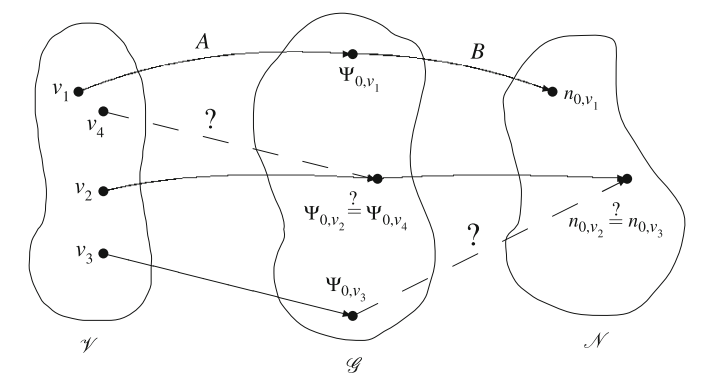
\includegraphics[width=0.55\textwidth]{bijekcija_med_v_psi_n.png}
  \caption{Bijection between the set of potentials, their corresponding ground
    states and ground state densities. Existance of such bijection is proved by
    Kohn-Sham theorems and proves that multi-particle system is
    uniquely determined by it's ground state particle density.}
  \label{bijection}
  \end{figure}

\end{document}